\chapter{Braids and the Jones polynomial}

\section{Motivation}

\adjustbox{scale=0.9,center}{
\begin{tikzcd}
	\centering
	& & {\begin{array}{@{}c@{}}\text{Jones} \\ \text{algebra}\end{array}} \arrow{r}{\text{\normalsize Markov}}[swap]{\text{\normalsize trace}} &[5em] {\begin{array}{@{}c@{}}\text{Jones} \\ \text{polynomial}\end{array}} \\
	{\begin{array}{@{}c@{}}\text{Oriented}\\ \text{link}\end{array}} \arrow[r] & {\begin{array}{@{}c@{}}\text{Artin} \\ \text{braid} \\ \text{group}\end{array}} \arrow[rd] \arrow[ru] & & \\
	& & {\begin{array}{@{}c@{}}\text{Temperley--} \\ \text{Lieb} \\ \text{algebra}\end{array}} \arrow{r}{\text{\normalsize Diagrammatic}}[swap]{\text{\normalsize trace}} &[5em] {\begin{array}{@{}c@{}}\text{Normalised}\\ \text{bracket}\\ \text{polynomial}\end{array}} \arrow[uu, leftrightarrow, sloped, above, "\text{\normalsize Substitution}"]
\end{tikzcd}}\vspace{10pt}

As remarked earlier, Jones arrived at his polynomial indirectly while working on the theory of operator algebras~\cite{jones}. In his course of investigations, he constructed a tower of algebras nested in one another with the property that each of these algebras is generated by a set of generators satisfying a particular set of relations. A degree of similarity between these relations and the relations among the generators of the \textit{Artin braid group} was pointed out to Jones by a student during a seminar~\cite[p.~216]{cromwell}, which led to the investigations of Jones into knot theory. Jones had defined a notion of a \textit{trace} on his algebras; more specifically a trace function obeying the \textit{Markov property}. As we shall see, one can express every link in terms of a (non-unique) \textit{braid}. Jones then defined a representation of such a braid into his algebras. The trace of an algebra representation of a braid, which is in turn obtained from the link, can be calculated. The Jones polynomial was realized as such a trace.

In this chapter, we shall not travel the original route of Jones to reach his polynomial as it requires the knowledge of the theory of von Neumann algebras. Instead, we shall follow the approach described by Kauffman in his book to construct a representation of the Artin braid group into the \textit{Temperley--Lieb algebra}~\cite[chp.~8]{kauffman}. These algebras admit a diagrammatic intrepretation and our definition of a trace on these algebras shall be diagrammatic in nature as well. Via this trace, we eventually reach the bracket polynomial, which we already know to be equivalent to the Jones polynomial as demonstrated earlier. The Jones algebra can be recovered from the Temperley--Lieb algebra by a choice of substitutions. The Temperley--Lieb algebra arose during the study of certain statistical models in physics~\cite{temperley-lieb}. This algebra can be viewed as a sub-algebra of a broader framework of the \textit{partition algebra}~\cite{partition-algebra}.

\section{Geometric representation of braids}

\subsection{Definition}

\begin{figure}
	\centering
	\begin{tikzpicture}
		[scale=1.5,
		cube/.style={thick,black},
		grid/.style={very thin,gray},
		axis/.style={->,blue,thick}]

		%draw a grid in the x-y plane
		%\foreach \x in {-0.5,0,...,2.5}
		%\foreach \y in {-0.5,0,...,2.5}
		%{
		%	\draw[grid] (\x,-0.5) -- (\x,2.5);
		%	\draw[grid] (-0.5,\y) -- (2.5,\y);
		%}

		%draw the axes
		\draw[axis] (0,0,0) -- (6,0,0) node[anchor=west]{\(x\)};
		\draw[axis] (0,0,0) -- (0,3,0) node[anchor=south]{\(y\)};
		\draw[axis] (0,0,0) -- (0,0,2) node[anchor=north east]{\(z\)};

		%draw the top and bottom of the cube
		\draw[cube] (0,0,-1) -- (0,2,-1) -- (5,2,-1) -- (5,0,-1) -- cycle;


		%draw the edges of the cube
		\draw[cube] (0,0,-1) -- (0,0,1);
		\draw[cube] (0,2,-1) -- (0,2,1);
		\draw[cube] (5,0,-1) -- (5,0,1);
		\draw[cube] (5,2,-1) -- (5,2,1);
% 		\draw[thick, black] (4,0,-1) -- (5,0,-1) -- (5,0,1) -- (4,0,1);

		\begin{knot}[clip width=8]
			\strand[thick, red] (1,0,0) to [in angle=-90, out angle=90, curve through = {(1.5,1,1)}] (4,2,0) node[black, below]{\(p_1\)};
			\strand[thick, red] (2,0,0) to [in angle=-90, out angle=90, curve through = {(1.7,1.5,0.5)}] (1,2,0) node[black, below]{\(p_2\)};
			\strand[thick, red] (3,0,0) to [in angle=-90, out angle=90, curve through = {(3,0.5,0.7)}] (2,2,0) node[black, below]{\(p_3\)};
			\strand[thick, red] (4,0,0) to [in angle=-90, out angle=90, curve through = {(3,1.3,-0.5)}] (3,2,0) node[black, below]{\(p_4\)};
			\flipcrossings{2}
		\end{knot}

		\node[below, label={\(q_1\)}] at (1,2,0) {};
		\node[below, label={\(q_2\)}] at (2,2,0) {};
		\node[below, label={\(q_3\)}] at (3,2,0) {};
		\node[below, label={\(q_4\)}] at (4,2,0) {};

		\draw[cube] (0,0,+1) -- (0,2,+1) -- (5,2,+1) -- (5,0,+1) -- cycle;

	\end{tikzpicture}
	\captionof{figure}{Three dimensional geometric representation of braids.}
	\label{fig:3drepbraids}
\end{figure}

We shall now understand some basics of braid theory. Emil Artin introduced the Artin braid group explicitly~\cite{artinzopfe, artin, friedman}.

An \(n\)-braid is an element of the Artin braid group \(\B_n\), defined via the following presentation on the generators \(\sigmaa_i\), for \(1 \leq i \leq n-1 \).
\[\B_n \coloneq\Biggl\langle
\begin{array}{c|rcll}
	& \sigmaa_i \sigmaa_i^{-1} &=& \symbb{I}_n^{\symrm{a}} &\\
	\sigmaa_1,\ldots, \sigmaa_{n-1} & \sigmaa_i \sigmaa_{i+1} \sigmaa_i &=& \sigmaa_{i+1} \sigmaa_i \sigmaa_{i+1} &\\
	& \sigmaa_i \sigmaa_j &=& \sigmaa_j \sigmaa_i &\text{if } \abs{i-j} \geq 2
\end{array}
\Biggr\rangle,\] where \(\symbb{I}_n^{\symrm{a}}\) is the identity of \(\B_n\).
Thus, \(\B_n\) is the quotient of the free group of \(n-1\) generators with the smallest normal subgroup of the free group containing the elements \(\sigmaa_i \sigmaa_i^{-1}\), \(\sigmaa_i \sigmaa_{i+1} \sigmaa_i \sigmaa_{i+1}^{-1} \sigmaa_i^{-1} \sigmaa_{i+1}^{-1}\) and \(\sigmaa_i \sigmaa_j \sigmaa_i^{-1} \sigmaa_{j}^{-1}\) with appropriately restricted \(i\) and \(j\). We want to recover this algebraic definition using the intuitive understanding of braids that we have. For, that we shall now see a geometric construction in the three dimensional Euclidean space to represent the Artin braid group. This shall make clear the geometric interpretation of the relations as well.

Consider two \textit{ordered} sets of points \(L_1 \coloneq \{p_1 \coloneq (1,0,0),\ldots, p_n \coloneq (n,0,0)\}\) and \(L_2 \coloneq \{q_1 \coloneq (1,1,0),\ldots, q_n \coloneq (n,1,0)\}\) as shown in \cref{fig:3drepbraids} for \(n=4\). Elements of \(L_1\) are called bottom points and elements of \(L_2\) are called the top points. For \(1 \leq i \leq n\), consider a family of non-intersecting continuous curves \(\gamma_i \colon [0, 1] \rightarrow \rthree\) such that
\begin{enumerate}
	\item \(\gamma_i (0) = p_i\) and \(\gamma_i (1) = q_j\) for \(1 \leq i, j \leq n\).
	\item Any plane perpendicular to the \(xy\)-plane and parallel to the \(x\)-axis intersects each of the curves either exactly once or not at all.
	\item All the curves lie in the cube determined by the vertices \((0,0,1)\), \((0,0,-1)\), \((0,1,1)\), \((0,1,-1)\), \((n+1,0,1)\), \((n+1,0,-1)\), \((n+1,1,1)\), \((n+1,1,-1)\).
\end{enumerate}
Such a labelled curve is called a strand in standard position and a family of such labelled \(n\) stands is called an \(n\)-strand set in a standard position. We can ambient isotope or rigidly move an \(n\)-strand set to get another \(n\)-strand set, possibly not in a standard position. Two \(n\)-strand sets are said to be equivalent if they are related by a sequence of rigid motions of the strand sets, and ambient isotopies of the strand sets such that the space outside the cube, along with the endpoints, remains fixed. We shall refer to an equivalence class of such \(n\)-strands as a geometric \(n\)-braid. Thus, a geometric \(n\)-braid is well-defined.

\begin{remark}
	Even though we have restricted our strands to the a bounded cube in the standard position, we can in principle change the bounds of our cube in \(x\) and \(z\) directions to any value and get the same theory. We shall not pursue this approach here.
\end{remark}

\subsection{Standard projection}

We call the projection of a standard position \(n\)-strand set onto the \(xy\)-plane to be a two dimensional representation of a braid. Such a projection is drawn in \cref{fig:2drepbraids}. It should be noted that a standard position \(n\)-strand set is unique only up to ambient isotopy, thus correspondingly the two dimensional representation of such a set is also unique only up to ambient isotopy, namely the ambient isotopies of the projection of the cube and the ambient isotopies such that the projection is a two dimensional representation of a braid for all times.

\begin{figure}
	\centering
	\begin{tikzpicture}
		[scale=1.5,
		cube/.style={thick,black},
		grid/.style={very thin,gray},
		axis/.style={->,blue,thick}]

		%draw a grid in the x-y plane
		%\foreach \x in {-0.5,0,...,2.5}
		%\foreach \y in {-0.5,0,...,2.5}
		%{
		%	\draw[grid] (\x,-0.5) -- (\x,2.5);
		%	\draw[grid] (-0.5,\y) -- (2.5,\y);
		%}

		%draw the axes
		\draw[axis] (0,0,0) -- (5,0) node[anchor=west]{\(x\)};
		\draw[axis] (0,0,0) -- (0,2.8) node[anchor=south]{\(y\)};

		\begin{knot}[clip width=8]
			\strand[thick, red] (1,0) to [in angle=-90, out angle=90, curve through = {(1.5,1)}] (4,2) node[black, below]{\(p_1\)};
			\strand[thick, red] (2,0) to [in angle=-90, out angle=90, curve through = {(1.7,1.5)}] (1,2) node[black, below]{\(p_2\)};
			\strand[thick, red] (3,0) to [in angle=-90, out angle=90, curve through = {(3,0.5)}] (2,2) node[black, below]{\(p_3\)};
			\strand[thick, red] (4,0) to [in angle=-90, out angle=90, curve through = {(3,1.3)}] (3,2) node[black, below]{\(p_4\)};
			\flipcrossings{2}
		\end{knot}

		\node[below, label={\(q_1\)}] at (1,2) {};
		\node[below, label={\(q_2\)}] at (2,2) {};
		\node[below, label={\(q_3\)}] at (3,2) {};
		\node[below, label={\(q_4\)}] at (4,2) {};
	\end{tikzpicture}
	\captionof{figure}{Two dimensional geometric representation of braids.}
	\label{fig:2drepbraids}
\end{figure}

Now onwards, we shall always visually represent geometric \(n\)-braids using their standard two dimensional projections.

\subsection{Group structure}

Multiplication of any two \(n\)-geometric braids \(b_1\) and \(b_2\), denoted by \(b_1 b_2\) is defined as follows (\cref{fig:braidmultiplication}). Ambient isotope and then rigidly move \(b_1\) and \(b_2\) \textit{separately} in the standard position. Now translate only \(b_1\) in the \(+y\) direction by unit distance. The bottom points of \(b_1\) and the top points of \(b_2\) now coincide. Concatenate their strands and shrink the concatenated strands in the \(y\) direction by half keeping fixed the bottom points of \(b_2\). The result is another geometric \(n\)-braid \(b_1 b_2\) in the standard position. Multiplication defined this way is associative.

\begin{figure}
	\centering
	\subcaptionbox[t]{\(b_1\)}{
		\begin{tikzpicture}
			[scale=1,
			cube/.style={thick,black},
			grid/.style={very thin,gray},
			axis/.style={->,blue,thick}]

			%draw a grid in the x-y plane
			%\foreach \x in {-0.5,0,...,2.5}
			%\foreach \y in {-0.5,0,...,2.5}
			%{
			%	\draw[grid] (\x,-0.5) -- (\x,2.5);
			%	\draw[grid] (-0.5,\y) -- (2.5,\y);
			%}

			%draw the axes
			\draw[axis] (0,0) -- (4,0) node[anchor=west]{\(x\)};
			\draw[axis] (0,0) -- (0,2.8) node[anchor=south]{\(y\)};

			\begin{knot}[clip width=5]
				\strand[thick, red] (1,0) to [in angle=-90, out angle=90, curve through = {(1.5,0.5)}] (1,2) node[black, below]{\(p_1\)\strut};
				\strand[thick, red] (2,0) to [in angle=-90, out angle=90, curve through = {(1.9,0.5)}] (3,2) node[black, below]{\(p_2\)\strut};
				\strand[thick, red] (3,0) to [in angle=-90, out angle=90, curve through = {(2,1.3)}] (2,2) node[black, below]{\(p_3\)\strut};
				\flipcrossings{2}
			\end{knot}

			%\node[below, label={\(q_1\)}] at (1,2) {};
			%\node[below, label={\(q_2\)}] at (2,2) {};
			%\node[below, label={\(q_3\)}] at (3,2) {};

			%\node at (2, -1.1) {\(b_1\)};
		\end{tikzpicture}\label{fig:braidmultiplication1}}\qquad
	\subcaptionbox[t]{\(b_2\)}{
		\begin{tikzpicture}
			[scale=1,
			cube/.style={thick,black},
			grid/.style={very thin,gray},
			axis/.style={->,blue,thick}]

			%draw a grid in the x-y plane
			%\foreach \x in {-0.5,0,...,2.5}
			%\foreach \y in {-0.5,0,...,2.5}
			%{
			%	\draw[grid] (\x,-0.5) -- (\x,2.5);
			%	\draw[grid] (-0.5,\y) -- (2.5,\y);
			%}

			%draw the axes
			\draw[axis] (0,0) -- (4,0) node[anchor=west]{\(x\)};
			\draw[axis] (0,0) -- (0,2.8) node[anchor=south]{\(y\)};

			\begin{knot}[clip width=5]
				\strand[thick, red] (1,0) to [in angle=-90, out angle=90, curve through = {(1.7,1)}] (2,2) node[black, below]{\(p_1'\)\strut};
				\strand[thick, red] (2,0) to [in angle=-90, out angle=90, curve through = {(1.7,0.5)}] (1,2) node[black, below]{\(p_2'\)\strut};
				\strand[thick, red] (3,0) to [in angle=-90, out angle=90, curve through = {(3,0.5)}] (3,2) node[black, below]{\(p_3'\)\strut};
			\end{knot}

			%\node[below, label={\(q_1'\)}] at (1,2) {};
			%\node[below, label={\(q_2'\)}] at (2,2) {};
			%\node[below, label={\(q_3'\)}] at (3,2) {};

			%\node at (2, -1.2) {\(b_2\)};
		\end{tikzpicture}\label{fig:braidmultiplication2}}
	\subcaptionbox[t]{\(b_1 b_2\)}{
		\begin{tikzpicture}
			[scale=1,
			cube/.style={thick,black},
			grid/.style={very thin,gray},
			axis/.style={->,blue,thick}]

			%draw a grid in the x-y plane
			%\foreach \x in {-0.5,0,...,2.5}
			%\foreach \y in {-0.5,0,...,2.5}
			%{
			%	\draw[grid] (\x,-0.5) -- (\x,2.5);
			%	\draw[grid] (-0.5,\y) -- (2.5,\y);
			%}

			%draw the axes
			\draw[axis] (0,0) -- (4,0) node[anchor=west]{\(x\)};
			\draw[axis] (0,0) -- (0,5) node[anchor=south]{\(y\)};

			\begin{knot}[clip width=5]
				\strand[thick, red] (1,0) to [in angle=-90, out angle=90, curve through = {(1.7,1)}] (2,2) node[black, below]{\(p_1''\)\strut};
				\strand[thick, red] (2,0) to [in angle=-90, out angle=90, curve through = {(1.7,0.5)}] (1,2) node[black, below]{\(p_2''\)\strut};
				\strand[thick, red] (3,0) to [in angle=-90, out angle=90, curve through = {(3,0.5)}] (3,2) node[black, below]{\(p_3''\)\strut};
				\strand[thick, red] (1,2) to [in angle=-90, out angle=90, curve through = {(1.5,2.5)}] (1,4);
				\strand[thick, red] (2,2) to [in angle=-90, out angle=90, curve through = {(1.9,2.5)}] (3,4);
				\strand[thick, red] (3,2) to [in angle=-90, out angle=90, curve through = {(2,3.3)}] (2,4);
				%\strand[thick, red] (1,0) to [in angle=-90, out angle=90, curve through = {(2,1)}] (3,4) node[black, below]{\(p_1\)};
				%\strand[thick, red] (2,0) to [in angle=-90, out angle=90, curve through = {(1,1)}] (1,4) node[black, below]{\(p_2\)};
				%\strand[thick, red] (3,0) to [in angle=-90, out angle=90, curve through = {(3,1)}] (2,4) node[black, below]{\(p_3\)};
				%\strand[thick, red] (1,2) to [in angle=-90, curve through = {(1.7,2)}] (2,4);
				%\strand[thick, red] (2,2) to [in angle=-90, curve through = {(1.7,1.5)}] (1,4) node[black, below];
				%\strand[thick, red] (3,2) to [in angle=-90, curve through = {(3,1.5)}] (3,4) node[black, below];
			\end{knot}

			%\node[below, label={\(q_1''\)}] at (1,4) {};
			%\node[below, label={\(q_2''\)}] at (2,4) {};
			%\node[below, label={\(q_3''\)}] at (3,4) {};

			%\node at (2, -1.2) {\(b_1 b_2\)};
		\end{tikzpicture}\label{fig:braidmultiplication3}}
	\caption{Multiplication of two braids (before shrinking).}\label{fig:braidmultiplication}
\end{figure}

We shall now drop the axes as well while representing two dimensional geometric \(n\)-braids.

An \(n\)-strand set such that each \(\gamma_i\) is a straight line segment connecting the \(i^\text{th}\) bottom point to the \(i^\text{th}\) top point is called the identity geometric \(n\)-braid and is denoted by \(\In\) (\cref{fig:braididentity}).

\begin{figure}\centering
	\begin{tikzpicture}
		[scale=0.7,
		cube/.style={thick,black},
		grid/.style={very thin,gray},
		axis/.style={->,blue,thick}]

		%draw a grid in the x-y plane
		%\foreach \x in {-0.5,0,...,2.5}
		%\foreach \y in {-0.5,0,...,2.5}
		%{
		%	\draw[grid] (\x,-0.5) -- (\x,2.5);
		%	\draw[grid] (-0.5,\y) -- (2.5,\y);
		%}

		%draw the axes
		\begin{knot}[clip width=5]
			\strand[thick, red] (1,0) to (1,2);
			\strand[thick, red] (2,0) to (2,2);
			\strand[thick, red] (3,0) to (3,2);
			\flipcrossings{2}
		\end{knot}

		\node[below, label={\(q_1\)}] at (1,2) {};
		\node[below, label={\(q_2\)}] at (2,2) {};
		\node[below, label={\(q_3\)}] at (3,2) {};
		\node[below, label={\(p_1\)}] at (1,-0.7) {};
		\node[below, label={\(p_2\)}] at (2,-0.7) {};
		\node[below, label={\(p_3\)}] at (3,-0.7) {};
	\end{tikzpicture}
	\captionof{figure}{The identity \(\I_3\)}
	\label{fig:braididentity}
\end{figure}

A geometric \(n\)-braid \(a\) such that \(ab = ba = \In\) for some geometric \(n\)-braid \(b\) is called the inverse of \(b\) and denoted is by \(b^{-1}\). We shall see that each element has an inverse.

With these operations, the set of geometric \(n\)-braids becomes a group, which we shall denote by \(\GB_n\).

\subsection{Generators}

By the virtue of ambient isotopy, we can move the crossings in a two dimensional representation of a geometric \(n\)-braid such that each crossing lies in a region bounded by two lines parallel to the \(x\)-axis. Moreover, we can arrange the crossings such that each such region contains only one crossing. Thus, if we give the information regarding the type of each crossing for each such region, we can faithfully reconstruct the two dimensional representation. To this end, we define the generators of a geometric \(n\)-braid.

Denote by \(\tauu_i\) the geometric \(n\)-braid such that
\begin{enumerate}
	\item \(\gamma_i (1) = q_{i+1}\), \(\gamma_{i+1} (1) = q_{i}\), and \(\gamma_j (1) = q_j\) when \(j\) does not equal \(i\) or \(i+1\).
	\item \(\pii_{xy}(\gamma_i(t)) \geq 0\) and \(\pii_{xy}(\gamma_{i+1}(t)) \leq 0\) for all \(t \in [0,1]\).
\end{enumerate}
\(\pii_{xy}\) is the projection maps onto to \(xy\)-plane. \(\tauu_1,\ldots, \tauu_{n-1}\) are the generators of \(\GB_n\) (\cref{fig:geometricbraidgenerators}).

\begin{figure}\centering
	\subcaptionbox{\(\tauu_i\)}{
		\begin{tikzpicture}
			[scale=0.7,
			cube/.style={thick,black},
			grid/.style={very thin,gray},
			axis/.style={->,blue,thick}]

			%draw a grid in the x-y plane
			%\foreach \x in {-0.5,0,...,2.5}
			%\foreach \y in {-0.5,0,...,2.5}
			%{
			%	\draw[grid] (\x,-0.5) -- (\x,2.5);
			%	\draw[grid] (-0.5,\y) -- (2.5,\y);
			%}

			%draw the axes
			\begin{knot}[clip width=8]
				\strand[thick, red] (0,0) to (2,2);
				\strand[thick, red] (2,0) to (0,2);
			\end{knot}

			\node[below, label={\(q_i\)}] at (0,2) {};
			\node[below, label={\(q_{i+1}\)}] at (2,2) {};
			\node[below, label={\(p_i\)}] at (0,-0.7) {};
			\node[below, label={\(p_{i+1}\)}] at (2,-0.7) {};

			%\node at (1, -1.1) {\(\tauu_i\)};
		\end{tikzpicture}}
	\qquad\quad\subcaptionbox{\(\tauu_i^{-1}\)}{
		\begin{tikzpicture}
			[scale=0.7,
			cube/.style={thick,black},
			grid/.style={very thin,gray},
			axis/.style={->,blue,thick}]

			%draw a grid in the x-y plane
			%\foreach \x in {-0.5,0,...,2.5}
			%\foreach \y in {-0.5,0,...,2.5}
			%{
			%	\draw[grid] (\x,-0.5) -- (\x,2.5);
			%	\draw[grid] (-0.5,\y) -- (2.5,\y);
			%}

			%draw the axes
			\begin{knot}[clip width=8]
				\strand[thick, red] (0,0) to (2,2);
				\strand[thick, red] (2,0) to (0,2);
				\flipcrossings{1}
			\end{knot}

			\node[below, label={\(q_i\)}] at (0,2) {};
			\node[below, label={\(q_{i+1}\)}] at (2,2) {};
			\node[below, label={\(p_i\)}] at (0,-0.7) {};
			\node[below, label={\(p_{i+1}\)}] at (2,-0.7) {};

			%\node at (1, -1.1) {\(\tauu_i^{-1}\)};
		\end{tikzpicture}}
	\caption{Generators \(\tauu_i\) and \(\tauu_i^{-1}\). We have omitted the other straight strands.}
	\label{fig:geometricbraidgenerators}
\end{figure}

\noindent For example, in \cref{fig:braidmultiplication} we have \(b_1 = \tauu_2 \in \GB_3\), \(b_2 = \tauu_1 \in \GB_3\) and \(b_1 b_2 = \tauu_2 \tauu_1 \in \GB_3\).

If we multiply \(\tauu_i\) and \(\tauu_i^{-1}\) to form \(\tauu_i \tauu_i^{-1}\), we observe that \(\tauu_i \tauu_i^{-1} = \I_n\), where \(\tauu_i, \tauu_i^{-1} \in \B_n\) for all \(n \geq 2\) (\cref{fig:type2}).

\begin{figure}\centering
	\begin{tikzpicture}
		[scale=0.7]

		\begin{knot}[clip width=5]
			\strand[thick, red] (0,0) to [in angle=-90, out angle=90, curve through = {(2,2)}] (0,4);
			\strand[thick, red] (2,0) to [in angle=-90, out angle=90, curve through = {(0,2)}] (2,4);
			\flipcrossings{1,2}
		\end{knot}

		\node at (1, -0.7) {\(\tauu_i \tauu_i^{-1}\)};
	\end{tikzpicture}
	\quad\quad\quad\quad
	\begin{tikzpicture}
		[scale=0.7]

		\begin{knot}[clip width=5]
			\strand[thick, red] (0,0) to (0,4);
			\strand[thick, red] (2,0) to (2,4);
			\flipcrossings{1,2}
		\end{knot}

		\node at (1, -0.7) {\(\I_n\)};
	\end{tikzpicture}

	\captionof{figure}{A type II move illustrating \(\tauu_i \tauu_i^{-1} = \I_n\)}
	\label{fig:type2}
\end{figure}

We can perform a move equivalent to the type III move to see that \(\tauu_i \tauu_{i+1} \tauu_i = \tauu_{i+1} \tauu_i \tauu_{i+1}\) (\cref{fig:type3}).

\begin{figure}\centering
	\begin{tikzpicture}
		[scale=0.6]

		\begin{knot}[clip width=5]
			\strand[ultra thick, blue] (0,0) to [in angle=-90, out angle=90, curve through = {(2,2) (4,4)}] (4,6);
			\strand[thick, red] (2,0) to [in angle=-90, out angle=90, curve through = {(0,2) (0,4)}] (2,6);
			\strand[thick, red] (4,0) to [in angle=-90, out angle=90, curve through = {(4,2) (2,4)}] (0,6);
		\end{knot}

		\node at (2, -0.7) {\(\tauu_i \tauu_{i+1} \tauu_i\)};
	\end{tikzpicture}
	\quad\quad\quad\quad
	\begin{tikzpicture}
		[scale=0.6]

		\begin{knot}[clip width=5]
			\strand[ultra thick, blue] (0,0) to [in angle=-90, out angle=90, curve through = {(0,2) (2,4)}] (4,6);
			\strand[thick, red] (2,0) to [in angle=-90, out angle=90, curve through = {(4,2) (2,4)}] (2,6);
			\strand[thick, red] (4,0) to [in angle=-90, out angle=90, curve through = {(2,2) (0,4)}] (0,6);
			%\flipcrossings{1,2}
		\end{knot}

		\node at (2, -0.7) {\(\tauu_{i+1} \tauu_i \tauu_{i+1}\)};
	\end{tikzpicture}

	\captionof{figure}{A type III move illustrating \(\tauu_i \tauu_{i+1} \tauu_i = \tauu_{i+1} \tauu_i \tauu_{i+1}\).}
	\label{fig:type3}
\end{figure}

We can slide two crossings vertically across each other if this does not change the ambient isotopy type. This is possible if the two crossings we wish to slide do not share a strand. This gives us the relation \(\tauu_i \tauu_j = \tauu_j \tauu_i\) if \(\abs{i - j} \geq 2\) (\cref{fig:sliding}).

\begin{figure}\centering
	\begin{tikzpicture}
		[scale=0.5]

		\begin{knot}[clip width=5]
			\strand[thick, red] (0,0) to [in angle=-90, out angle=90, curve through = {(2,2)}] (2,6);
			\strand[thick, red] (2,0) to [in angle=-90, out angle=90, curve through = {(0,2)}] (0,6);
			\strand[thick, red] (4,0) to [in angle=-90, out angle=90, curve through = {(4,4)}] (6,6);
			\strand[thick, red] (6,0) to [in angle=-90, out angle=90, curve through = {(6,4)}] (4,6);
		\end{knot}

		\node at (3, -0.7) {\(\tauu_i \tauu_j\)};
	\end{tikzpicture}
	\quad\quad\quad\quad
	\begin{tikzpicture}
		[scale=0.5]

		\begin{knot}[clip width=5]
			\strand[thick, red] (0,0) to [in angle=-90, out angle=90, curve through = {(0,4)}] (2,6);
			\strand[thick, red] (2,0) to [in angle=-90, out angle=90, curve through = {(2,4)}] (0,6);
			\strand[thick, red] (4,0) to [in angle=-90, out angle=90, curve through = {(6,2)}] (6,6);
			\strand[thick, red] (6,0) to [in angle=-90, out angle=90, curve through = {(4,2)}] (4,6);
			%\flipcrossings{1,2}
		\end{knot}

		\node at (3, -0.7) {\(\tauu_j \tauu_i\)};
	\end{tikzpicture}

	\captionof{figure}{Sliding of crossings illustrating \(\tauu_i \tauu_j = \tauu_j \tauu_i\).}
	\label{fig:sliding}
\end{figure}

Let \(w\) be a word of length \(m\) in \(\GB_n\); \(w = \prod_{j=1}^{m} \tauu^{\pm 1}_{\alpha_j}\) where \(1 \leq \alpha_j \leq n-1\). Every element of \(\GB_n\) and \(\B_n\) can be expressed as a product of its generators, albeit non-uniquely. We define a homomorphism
\begin{align*}
	\upPhi &\colon \GB_n \rightarrow \B_n,\\
	\upPhi &\colon \prod_{j=1}^{m} \tauu^{\pm 1}_{\alpha_j} \mapsto \prod_{j=1}^{m} \sigmaa^{\pm 1}_{\alpha_j} \text{ for all } m \in \symbb{N}.
\end{align*}

\noindent We can see that \(\upPhi\) is a surjection as follows. Take an element \(\prod_{j=1}^{m} \sigmaa^{\pm 1}_{\alpha_j} \in \B_n\), \(\upPhi\) maps \(\prod_{j=1}^{m} \tauu^{\pm 1}_{\alpha_j}\) to \(\prod_{j=1}^{m}\sigmaa^{\pm 1}_{\alpha_j}\). Proving that \(\upPhi\) is an injection is harder and a proof can be found in ~\cite[chp.~2]{murasugibraids}.
\begin{thm}
    \(\upPhi\) is an isomorphism, i.e.\@ \(\B_n\) and \(\GB_n\) are isomorphic.
\end{thm}
\noindent This allows us to forget the distinction between \(\B_n\) and \(\GB_n\).

\section{Closure of braids}

We define the closure of a geometric \(n\)-braid as follows. Consider a geometric \(n\)-braid in the standard position. For each \(1 \leq i \leq n\), we construct the following sequence of line connected line segments. Join \((i, 1, 0)\), \((i, i, 0)\), \((i, i, 0)\), \((i, -i, 0)\), \((i, -i, 0)\), \((i, 0, 0)\) consecutively. We then join \(\gamma_i\) to the constructed line segments. Repeating this process for all \(i\) gives the closure of a braid (\cref{fig:closure}). We denote the closure of a geometric \(n\)-braid \(b\) by \(\overline{b}\). Closure of a braid is unique up to ambient isotopy. Two equivalent braid words have the same closures, thus making the closure well-defined.

\begin{figure}\centering
	\subcaptionbox{\(b\)}{
		\begin{tikzpicture}
			[scale=0.6]

			\begin{knot}[clip width=5]
				\strand[very thick, blue] (0,0) to[in angle=-90, out angle=90, curve through = {(1,1)}] (2,2);
				\strand[very thick, blue] (2,0) to[in angle=-90, out angle=90, curve through = {(1,1)}] (0,2);
				\strand[very thick, blue] (4,0) to (4,2);
				%\strand[thick, red] (6,0) to [in angle=-90, out angle=90, curve through = {(6,4)}] (4,6);
			\end{knot}

			%\node at (2, -0.7) {\(b\)};\cite{witten}
		\end{tikzpicture}}
	\quad\quad\subcaptionbox{\(\overline{b}\)}{
		\begin{tikzpicture}
			[scale=0.6]

			\begin{knot}[clip width=5]
				\strand[very thick, blue] (0,0) to[in angle=-90, out angle=90, curve through = {(1,1)}] (2,2);
				\strand[very thick, blue] (2,0) to[in angle=-90, out angle=90, curve through = {(1,1)}] (0,2);
				\strand[very thick, blue] (4,0) to (4,2);
				\strand[thick, red] (4,2) to (4,3) to (5,3) to (5,-1) to (4,-1) to (4,0);
				\strand[thick, red] (2,2) to (2,4) to (6,4) to (6,-2) to (2,-2) to (2,0);
				\strand[thick, red] (0,2) to (0,5) to (7,5) to (7,-3) to (0,-3) to (0,0);
				%\strand[thick, red] (0,4) t
				%\flipcrossings{1,2}
			\end{knot}

			%\node at (5, -6.7) {\(\overline{b}\)};
		\end{tikzpicture}}
	\caption{Closure of a braid with \(b = \tauu_1 \in \GB_2\).}
	\label{fig:closure}
\end{figure}

\begin{prop}
	Every closure of a geometric \(n\)-braid is a link.
\end{prop}
\begin{proof}[Proof]
	The outer line segments are locally flat by virtue of being piecewise linear. Due to the second condition regarding the intersection of a plane in the standard representation of geometric \(n\)-braid, we can project the strand onto the \(y\)-axis and this projection would be a homeomorphism. We take an \(\epsilon\) neighbourhood, \(N(\epsilon)\) around the strand. The pair \((N(\epsilon), \gamma_i)\) would then be homeomorphic to \((\symup{B}, \symup{B} \cap x\text{-axis})\), where \(\symup{B}\) is the three-dimensional unit ball around the origin. We have local flatness at the end points as well due to the union of two locally flat curves.
\end{proof}

\begin{remark}
	Suppose \(\tauu_i \in \GB_n\) and \(\tauu_i' \in \GB_{m}\) are generators where \(n < m\). Then the closures of these two generators are not ambient isotopic. The closure of the latter contains one more non-linking loop.
\end{remark}
\subsection{Alexander Theorem}

The theorems of James Alexander~\cite{alexander} and Andrei Markov Jr.~\cite{markov} relate braids to knots.

\begin{thm}[Alexander]
	Every link is ambient isotopic to the closure of a geometric braid, for some \(n \in \symbb{N}\).
\end{thm}
\begin{proof}
	Consider a piecewise linear, regular projection \(\symup{\pi}(L)\) of a link \(L\) on a plane. We choose a point \(O\) in the projection plane which is not collinear with any of the line segments. This can be done since a the link has only finitely many line segments. Let \(P \in \symup{\pi}(L)\). The vector \(OP\) can move either clockwise or anti-clockwise as \(P\) moves along the link projection. We wish to modify the line segments such that \(OP\) moves in only one sense, say anti-clockwise, as \(P\) moves along the entire length of the link projection. We now fix our attention on a line segment corresponding to a clockwise rotation. We divide the segment into sub-parts such that each part shares at-most one crossing point with other line segments. If \(A\) and \(B\) are end-points of such a line segment, then we may replace this line segment with two another line segments \(AC\) and \(CB\), such that \(C\) is another point not on belonging to \(\symup{\pi}(L)\) and the triangle \(ABC\) encloses \(O\). If \(AB\) originally passed under (or over) a line segment of \(\symup{\pi}(L)\), then the modified line segments \(AC\) and \(CB\) must pass under (or over) of the line segments of \(\symup{\pi}(L)\) as well. This move shall not change the link type as it shall be a combination of sliding, type 2 and type 3 moves. In the resulting triangle, we have two orientations possible, one path which travels via \(C\) and the other path which does not. The vector \(OP\) shall move in the opposite, anti-clockwise sense while traversing from \(A\) to \(B\) via \(C\), instead of \(AB\). We can repeat this process for all of the (finitely many) line segments which turn clockwise. In the end, we obtain a projection such that \(OP\) moves in only the anti-clockwise sense, as \(P\) moves along the entire length of the link projection. We can ambient isotope the projection such that all the crossings lie in the projection of a cube, more precisely the cube constructed while defining a geometric braid. The end-points can be made to match as well. The above procedure of triangular moves shall guarantee the monotonicity that is required.
\end{proof}

Henceforth, unless specified otherwise, we shall always work with the projections of the standard representation of a geometric \(n\)-braid and its closure and refer to these projections simply as a braid and its closure.

\subsection{Conjugation}

If \(b, g \in \GB_n\), we observe that \(\overline{g b g^{-1}}\) is ambient isotopic to \(\overline{b}\) (\cref{fig:conjugation}). The upper strands in \(g\) and \(g^{-1}\) are connected via the closure strand. We can slide \(g\) and \(g^{-1}\) via the closure strands to the `other side' of \(b\) to annihilate each other. This can be achieved by a type II move.

\begin{figure}
	\centering
	\subcaptionbox{}{
		\begin{tikzpicture}
			\begin{knot}[clip width = 5]
				\strand[thick, red] (0,0) to [in=-90, out=90](1,1);
				\strand[thick, red] (0,2) to [out=90, in=-90](1,3) to (1,3.5) to (1.5,3.5) to (1.5,-0.5) to (1,-0.5) to (1,0);
				\strand[thick, red] (1,0) to [in=-90, out=90](0,1);
				\strand[thick, red] (1,2) to [out=90, in=-90](0,3) to (0,4) to (2,4) to (2,-1) to (0,-1) to (0,0);
				\strand[very thick, blue] (1,1) to [out=90,in=-90, blue] (0,2);
				\strand[very thick, blue] (0,1) to [out=90,in=-90, blue] (1,2);
				\flipcrossings{2}
			\end{knot}
			\node at (-0.5,0.5) {\(g^{-1}\)};
			\node at (-0.5,1.5) {\(b\)};
			\node at (-0.5,2.5) {\(g\)};
		\end{tikzpicture}}
	\quad\quad\subcaptionbox{}{
		\begin{tikzpicture}
			\begin{knot}[clip width = 5]
				\strand[thick, red] (0,2) to (0,3.5) to (1.5,3.5) to (2.5,2.5) to (3,2.5) to (3,0.5) to (2.5,0.5) to (1.5,-0.5) to (0,-0.5) to (0,1);
				\strand[thick, red] (1,2) to (1,2.5) to (1.5,2.5) to (2.5,3.5) to (3.5,3.5) to (3.5,-0.5) to (2.5,-0.5) to (1.5,0.5) to (1,0.5) to (1,1);
				\strand[very thick, blue] (1,1) to [out=90,in=-90, blue] (0,2);
				\strand[very thick, blue] (0,1) to [out=90,in=-90, blue] (1,2);
				\flipcrossings{1,2}
			\end{knot}
			\node at (2,-1) {\(g^{-1}\)};
			\node at (-0.5,1.5) {\(b\)};
			\node at (2,4) {\(g\)};
		\end{tikzpicture}}\par\bigskip
	\subcaptionbox{}{
		\begin{tikzpicture}
			\begin{knot}[clip width = 5]
				\strand[thick, red] (0,2) to (0,3.75) to (2.5,3.75) to (2.5,2.75) to (1.5,1.75) to (1.5,1.25) to (2.5,0.25) to (2.5,-0.75) to (0,-0.75) to (0,1);
				\strand[thick, red] (1,2) to (1,3.25) to (1.5,3.25) to (1.5,2.75) to (2.5,1.75) to (2.5,1.25) to (1.5,0.25) to (1.5,-0.25) to (1,-0.25) to (1,1);
				\strand[very thick, blue] (1,1) to [out=90,in=-90, blue] (0,2);
				\strand[very thick, blue] (0,1) to [out=90,in=-90, blue] (1,2);
				\flipcrossings{1,2}
			\end{knot}
			\node at (3,0.75) {\(g^{-1}\)};
			\node at (-0.5,1.5) {\(b\)};
			\node at (3,2.25) {\(g\)};
		\end{tikzpicture}}
	\quad\quad\subcaptionbox{}{
		\begin{tikzpicture}
			\begin{knot}[clip width = 5]
				\strand[thick, red] (0,2) to (0,3) to (2,3) to (2,0) to (0,0) to (0,1);
				\strand[thick, red] (1,2) to (1,2.5) to (1.5,2.5) to (1.5,0.5) to (1,0.5) to (1,1);
				\strand[very thick, blue] (1,1) to [out=90,in=-90, blue] (0,2);
				\strand[very thick, blue] (0,1) to [out=90,in=-90, blue] (1,2);
				\flipcrossings{1,2}
			\end{knot}
			\node at (-0.5,1.5) {\(b\)};
		\end{tikzpicture}}
	\caption{Conjugation process illustrating the link equivalence of \(\overline{g b g^{-1}}\) and \(\overline{b}\), with \(b = \tauu_1^{-1} \in \GB_1\) and \(g = \tauu_1^{-1} \in \GB_1\).}
	\label{fig:conjugation}
\end{figure}

\begin{remark}
	The closures of conjugate braids are ambient isotopic as links. The braids themselves are not.
\end{remark}

\subsection{Markov move}

We observe that if \(b \in \GB_n\), then \(b \tauu_n \in \GB_{n+1}\), \(b \tauu_n^{-1} \in \GB_{n+1}\) and \(b\) have ambient isotopic closures (\cref{fig:markovmove}), although \(b\), \(b\tauu_n\) and \(b\tauu_n^{-1}\) are not equivalent as braids. That is, we can add a strand and a crossing of that strand with another strand without changing the link type (of the closure). We can also remove a strand and a crossing if that strand does not cross any other strand. We visually see that adding the above mentioned strands anywhere between the existing strands is equivalent to adding the strands on the right.

\begin{figure}
	\centering
	\subcaptionbox{\(\overline{b}\)}{
		\begin{tikzpicture}
			\begin{knot}[clip width = 5]
				\strand[thick, red] (0,2) to (0,3) to (2,3) to (2,0) to (0,0) to (0,1);
				\strand[thick, red] (1,2) to (1,2.5) to (1.5,2.5) to (1.5,0.5) to (1,0.5) to (1,1);
				\strand[very thick, blue] (1,1) to [out=90,in=-90, blue] (0,2);
				\strand[very thick, blue] (0,1) to [out=90,in=-90, blue] (1,2);
				\flipcrossings{2}
			\end{knot}
			\node at (-0.5,1.5) {\(b\)};
		\end{tikzpicture}}
	\quad\quad\subcaptionbox{\(\overline{b\tauu_2}\)}{
		\begin{tikzpicture}
			\begin{knot}[clip width = 5]
				\strand[very thick, blue] (0,0) to (0,1) to [out=90,in=-90, blue] (1,2);
				\strand[thick, red] (1,2) to (1,3) to (3,3) to (3,-1) to (1,-1) to (1,0);
				\strand[very thick, blue] (1,0) to [out=90,in=-90, blue] (2,1) to (2,2);
				\strand[thick, red] (2,2) to (2,2.5) to (2.5,2.5) to (2.5,-0.5) to (2,-0.5) to (2,0);
				\strand[very thick, blue] (2,0) to [out=90,in=-90, blue]  (1,1) to [out=90,in=-90, blue] (0,2);
				\strand[thick, red] (0,2) to (0,3.5) to (3.5,3.5) to (3.5,-1.5) to (0,-1.5) to (0,0);
				\flipcrossings{1}
			\end{knot}
		\end{tikzpicture}}
	\caption{Markov move with \(b = \tauu_1^{-1}\).}
	\label{fig:markovmove}
\end{figure}

\subsection{Markov Theorem}

\begin{thm}[Markov]
	Two braids whose closures are ambient isotopic to each other are related by a finite sequence of the following operations.
	\begin{enumerate}
		\item Braid equivalences, i.e.\@ equivalences resulting due to the braid relations.
		\item Conjugation.
		\item Markov moves.
	\end{enumerate}
\end{thm}
\noindent A proof of the above theorem can be found in the book of Joan Birman~\cite[chp.~2]{birman}. Markov gave a sketch of the proof in 1936~\cite{markov}.

\subsection{Writhe}

We see visually that the result of a Markov move on a braid is equivalent to performing a type I move on the braid closure. We know that a type I move increases or decreases the writhe of a link by a unit value. Since all the crossings in a braid closure occur only in the cube containing the braid strands, we can define the writhe of a braid equal to the writhe of the braid closure by assigning each braid crossing a value, either \(+1\) or \(-1\). Our assignment must be consistent with our earlier assignment for knots. But for this procedure, we need to assign an orientation to the braid. We assign all the strands (inside the braid cube) a downward orientation. Doing so, we see that \(\tauu_i\) inherits \(+1\) value while \(\tauu_i^{-1}\) inherits \(-1\). We could instead have assigned all the strands an upward orientation as well. This would not have changed the values of \(\tauu_i\) and \(\tauu_i^{-1}\) (\cref{fig:writhebraids}). What is not allowed is assigning arbitrary orientation to strands. If we assign the orientation arbitrarily, then the well-definedness of the orientation cannot be guaranteed. Two distinct strands in a braid could be connected via the closure strands and one would need to check the whole connected link component of the braid closure for a well-defined closure.

\noindent Thus, the writhe \(w\) of the braid \(b\) with a word representation \(\prod_{j=1}^{m} \tauu^{\beta_j}_{\alpha_j}\) of length \(m\), where \(\beta_j \in \{+1, -1\}\) is \[w(b) = \sum_{j = 1}^{m}\beta_j.\] Note that the writhe of a braid is dependent on its word representation. We also see that \(w(b) = w(\overline{b})\).

\begin{figure}
	\centering
	\subcaptionbox{}{
		\begin{tikzpicture}
			\begin{knot}[clip width = 5]
				\strand[<-, thick, red] (1,1) to (0,2);
				\strand[<-, thick, red] (0,1) to (1,2);
				\flipcrossings{1}
			\end{knot}
		\end{tikzpicture}}\label{a}\quad
	\subcaptionbox{}{
		\begin{tikzpicture}
			\begin{knot}[clip width = 5]
				\strand[->, thick, red] (1,1) to (0,2);
				\strand[->, thick, red] (0,1) to (1,2);
				\flipcrossings{1}
			\end{knot}
		\end{tikzpicture}}\label{b}\quad
	\subcaptionbox{}{
		\begin{tikzpicture}
			\begin{knot}[clip width = 5]
				\strand[<-, thick, red] (1,1) to (0,2);
				\strand[<-, thick, red] (0,1) to (1,2);
			\end{knot}
		\end{tikzpicture}}\label{c}\quad
	\subcaptionbox{}{
		\begin{tikzpicture}
			\begin{knot}[clip width = 5]
				\strand[->, thick, red] (1,1) to (0,2);
				\strand[->, thick, red] (0,1) to (1,2);
			\end{knot}
		\end{tikzpicture}}\label{d}
	\caption{Assignment of crossing values. (a) Downward orientation for \(\tauu_i\) corresponding to \(+1\). (b) Upward orientation for \(\tauu_i\) corresponding to \(+1\). (c) Downward orientation for \(\tauu_i^{-1}\) corresponding to \(-1\). (d) Upward orientation for \(\tauu_i^{-1}\) corresponding to \(-1\).}
	\label{fig:writhebraids}
\end{figure}

\section{Markov trace}

We won't distinguish between \(\B_n\) and \(\GB_n\) from now on. We can now move finally towards the Jones/bracket polynomial with the information we have. If we have a function \(J_n \colon \B_n \rightarrow R\), where \(R\) is a commutative ring, then using the Markov Theorem we can construct link invariants from the family of functions \(\{J_n\}\) if the following conditions are satisfied.
\begin{enumerate}
    \item \(J_n\) is well defined. \(J_n(b)\) = \(J_n(b')\) if \(b = b'\).
	\item \(J_n(b) = J_n(gbg^{-1})\) if \(g, b \in \B_n\).
	\item If \(b \in \B_n\), then there exists a constant \(\alpha\in R\), independent of \(n\), such that \[J_{n+1} (b\sigma_n) = \alpha^{+1} J_n(b)\] and \[J_{n+1} (b\sigma_{n}^{-1}) = \alpha^{-1} J_n(b).\]
\end{enumerate}
\noindent The last condition reminds us of the normalisation needed in order to make the bracket polynomial invariant under the type I move. Its purpose here is the same.

A family of functions \(\{J_n\}\) satisfying the above given three conditions is called a Markov trace on \(\{\B_n\}\). For any link \(L\) which is ambient isotopic to \(\overline{b}\), where \(b \in \B_n\), we define \(J(L) \in R\) as follows. \[J(L) \coloneq \alpha^{-w(b)}J_n(b).\] We call \(J(L)\) the link invariant for the Markov trace \(\{J_n\}\).

\begin{thm}
    \(J\) is an invariant of ambient isotopy for oriented links.
\end{thm}
\begin{proof}
	Suppose \(L \sim \overline{b}\) and \(L'' \sim \overline{b'}\), where \(\sim\) denotes the ambient isotopy relation. By the Markov Theorem, we can obtain \(\overline{b'}\) via an application of a finite sequence of the moves mentioned in the Markov Theorem  on \(\overline{b'}\). Each such move leaves \(J\) invariant. \(J_n\) is already invariant under braid equivalences and conjugation by definition. The \(\alpha^{-w(b)}\) factor cancels the effect of a type I move.
\end{proof}

We can define the bracket polynomial for braids in the same way as we did for links. Define
\begin{align*}
	\langle \cdot \rangle &\colon \B_n \rightarrow \z[A, A^{-1}]\\
	\langle \cdot \rangle &\colon b \mapsto \langle \overline{b}\rangle.
\end{align*}
We simply evaluate the bracket on the closure of the braid. We observe that this function is a Markov trace with \(\alpha = -A^{3}\). We know that \[\BB = A\BD + A^{-1}\BE.\] In terms of braids, we have \[\left\langle\BPB\right\rangle = A\left\langle\BPD\right\rangle + A^{-1}\left\langle\BPE\right\rangle.\] But \(\BPE\) is the identity braid. Thus, if we denote \(\BPD\) by \(\symup{U}_i\), we can write \[\left\langle{\sigmaa_{i}^{-1}}\right\rangle = A\braket<\symup{U}_i> + A^{-1}\braket<\I_n>.\] Similarly, one could write \[\braket<\sigmaa_i> = A\braket<\I_n> + A^{-1}\braket<\symup{U}_i>.\] Note that \(\symup{U}_i\) does not belong to the braid group and is a new object. We refer to them as ``input-output forms'' or as ``hooks''. They are cup and cap combinations involving the \(i\)-th and \((i+1)\)-th strands (\cref{fig:inputoutputforms}).
\begin{figure}
    \centering
	\subcaptionbox{\(U_1\)}{
		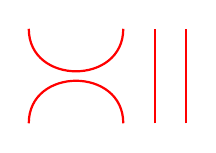
\begin{tikzpicture}[scale=2]
			\draw[thick, red] (-0.3,0.3) .. controls (-0.3,-0.06) and (0.3,-0.06) .. (0.3,0.3);
			\draw[thick, red] (-0.3,-0.3) .. controls (-0.3,0.06) and (0.3,0.06) .. (0.3,-0.3);
			\draw[thick, red] (0.5,-0.3) -- (0.5,0.3);
			\draw[thick, red] (0.7,-0.3) -- (0.7,0.3);
		\end{tikzpicture}}
	\quad\quad\quad\subcaptionbox{\(U_2\)}{
		\begin{tikzpicture}[scale=2]
			\begin{knot}[clip width = 5]
				\draw[thick, red] (-0.5,-0.3) -- (-0.5,0.3);
				\draw[thick, red] (-0.3,0.3) .. controls (-0.3,-0.06) and (0.3,-0.06) .. (0.3,0.3);
				\draw[thick, red] (-0.3,-0.3) .. controls (-0.3,0.06) and (0.3,0.06) .. (0.3,-0.3);
				\draw[thick, red] (0.5,-0.3) -- (0.5,0.3);
			\end{knot}
		\end{tikzpicture}}
	\quad\quad\quad\subcaptionbox{\(U_3\)}{
		\begin{tikzpicture}[scale=2]
			\begin{knot}[clip width = 5]
				\draw[thick, red] (-0.5,-0.3) -- (-0.5,0.3);
				\draw[thick, red] (-0.3,0.3) .. controls (-0.3,-0.06) and (0.3,-0.06) .. (0.3,0.3);
				\draw[thick, red] (-0.3,-0.3) .. controls (-0.3,0.06) and (0.3,0.06) .. (0.3,-0.3);
				\draw[thick, red] (-0.7,-0.3) -- (-0.7,0.3);
			\end{knot}
		\end{tikzpicture}}
	\caption{Input-output forms or hooks for 4 strands}
	\label{fig:inputoutputforms}
\end{figure}
We can thus use consider \(\sigmaa_i\) to be equivalent to \(A + A^{-1}\symup{U}_i\), \(\sigmaa^{-1}_i\) to be equivalent to \(A^{-1} + A\symup{U}_i\), and create a formalism based on this. Given a braid word representation of a braid, we can simply substitute the above mentioned equivalences to get a product of \(\symup{U}_i\)'s, with \(A\) and \(A^{-1}\) as coefficients. Note that this product is dependent on the specific braid representation of a knot. It is not invariant under a type I move, as is the case with the un-normalised bracket polynomial.

We see that each bracket polynomial evaluation state of the closure of a braid can be written in terms of the closure of a product of the input-output forms. Given a braid word \(b\), we can consider it equivalent to \(S(b)\), where \(S(b)\) is the sum of products of the \(\symup{U}_i\)'s obtained by substituting \(\sigmaa_i\) by \(A + A^{-1}\symup{U}_i\) and \(\sigmaa_i^{-1}\) by \(A^{-1} + A\symup{U}_i\). Closure of each term (a product in \(U_i\)'s) in the sum corresponds to a state obtained while evaluating the bracket polynomial as it gives a collection of loops. If \(P\) is such a product, then \(\left\langle P\,\right\rangle = \braket<\overline{P}\,> = \symup{\delta}^{\norm{P}}\), where \(\norm{P}\) is the number of loops in \(\overline{P}\) minus \(1\), and \(\symup{\delta} = -A^{-2} - A^2\). Thus, \[S(b) = \sum_s \braket<b|s> P_s,\] where \(s\) denotes a state and indexes all the terms in the product, and \(\braket<b|s>\) is the product of \(A\)'s and \(A^{-1}\)'s multiplying each \(P\)-product \(P_s\). We have \[\braket<b> = \braket<S(b)> = \sum_s \braket<b|s> \braket<P_s> = \sum_s \braket<b|s> \updelta^{\norm{s}}.\]

\begin{exmp}
	Let \(b = \sigmaa_1\sigmaa_2^{-1}\). We can resolve \(\overline{b}\) in many states. One of the states \(s\) and its corresponding product \(\U_1 \U_2\) in terms of the input-output forms is shown in \cref{fig:inputoutputexample}.
	\begin{figure}
	    \centering
		\subcaptionbox{\(b\)}{
			\begin{tikzpicture}
				\begin{knot}[clip width=5]
					\strand[very thick, blue] (2,0) to [out=90,in=-90] (1,1);
					\strand[very thick, blue] (1,1) [out=90,in=-90] to (0,2);
					\strand[very thick, blue] (1,0) to [out=90,in=-90] (2,1);
					\strand[very thick, blue] (2,1) [out=90,in=-90] to (2,2);
					\strand[very thick, blue] (0,0) to [out=90,in=-90] (0,1);
					\strand[very thick, blue] (0,1) [out=90,in=-90] to (1,2);
					\flipcrossings{2}
				\end{knot}
			\end{tikzpicture}}
		\quad\quad\subcaptionbox{\(\overline{b}\)}{
			\begin{tikzpicture}
				\begin{knot}[clip width=5]
					\strand[very thick, blue] (2,0) to [out=90,in=-90] (1,1);
					\strand[very thick, blue] (1,1) [out=90,in=-90] to (0,2);
					\strand[very thick, blue] (1,0) to [out=90,in=-90] (2,1);
					\strand[very thick, blue] (2,1) [out=90,in=-90] to (2,2);
					\strand[very thick, blue] (0,0) to [out=90,in=-90] (0,1);
					\strand[very thick, blue] (0,1) [out=90,in=-90] to (1,2);
					\strand[thick, red] (2,2) to (2,2.5) to (2.5, 2.5) to (2.5,-0.5) to (2,-0.5) to (2,0);
					\strand[thick, red] (1,2) to (1,3) to (3,3) to (3,-1) to (1,-1) to (1,0);
					\strand[thick, red] (0,2) to (0,3.5) to (3.5,3.5) to (3.5,-1.5) to (0,-1.5) to (0,0);
					\flipcrossings{2}
				\end{knot}
			\end{tikzpicture}}\par\bigskip
		\subcaptionbox{\(s = \overline{U_1 U_2}\)}{
			\begin{tikzpicture}
				\begin{knot}[clip width=5]
					\draw[very thick, blue] (1,0) .. controls (1,0.5) and (2,0.5) .. (2,0);
					\draw[very thick, blue] (1,1) .. controls (1,0.5) and (2,0.5) .. (2,1) to (2,2);
					\draw[very thick, blue] (0,0) to (0,1) .. controls (0,1.5) and (1,1.5) .. (1,1);
					\draw[very thick, blue] (0,2) .. controls (0,1.5) and (1,1.5) .. (1,2);
					\strand[thick, red] (2,2) to (2,2.5) to (2.5, 2.5) to (2.5,-0.5) to (2,-0.5) to (2,0);
					\strand[thick, red] (1,2) to (1,3) to (3,3) to (3,-1) to (1,-1) to (1,0);
					\strand[thick, red] (0,2) to (0,3.5) to (3.5,3.5) to (3.5,-1.5) to (0,-1.5) to (0,0);
				\end{knot}
			\end{tikzpicture}}
		\quad\quad\quad\subcaptionbox{\(U_1 U_2\)}{
			\begin{tikzpicture}
				\begin{knot}[clip width=5]
					\draw[very thick, blue] (1,0) .. controls (1,0.5) and (2,0.5) .. (2,0);
					\draw[very thick, blue] (1,1) .. controls (1,0.5) and (2,0.5) .. (2,1) to (2,2);
					\draw[very thick, blue] (0,0) to (0,1) .. controls (0,1.5) and (1,1.5) .. (1,1);
					\draw[very thick, blue] (0,2) .. controls (0,1.5) and (1,1.5) .. (1,2);
				\end{knot}
			\end{tikzpicture}}
		\caption{Writing a state of a braid closure in terms of input-output forms.}
		\label{fig:inputoutputexample}
	\end{figure}
\end{exmp}

\begin{exmp}
	Consider the same braid \(b = \sigmaa_1\sigmaa^{-1}_2\). We have
	\begin{align*}
	    P(b) &= (A + A^{-1}\U_1) (A\U_2 + A^{-1})\\
		P(b) &= A^2\U_2 + \I_3 + \U_1\U_2 + A^{-2}\U_1\\
		\braket<b> = \braket<\sigmaa_1\sigmaa^{-1}_2> = \braket<P(b)> &= A^2\braket<\U_2> + \braket<\I_3> + \braket<\U_1\U_2> + A^{-2}\braket<\U_1>.
	\end{align*}
	Now, \(\I_3\) corresponds to \BPIthree. Thus, \(\braket<I_3> = \updelta^{3-1} = \updelta^2\) as the closure of \(\I_3\) shall give three loops. \(\U_1\) corresponds to \KPDonethree\,. Thus, \(\braket<\U_1> = \updelta^{2-1} = \updelta\) as the closure shall give two loops. Similarly, \(\braket<\U_2> = \updelta\) and \(\braket<\U_1\U_2> = \updelta^{1-1} = 1.\) For a visual representation of the state \(\U_1\U_2\), see \cref{fig:inputoutputexample}, where the closure gives one single loop. In the end, we get \[\braket<\overline{b}> = A^2\updelta + \updelta^2 + 1 + A^{-2}\updelta.\]
\end{exmp}

\section{Temperley--Lieb algebra}

We can give the \(\U_i\)'s a structure of their own by constructing the free additive algebra \(\TL_n\) with the generators \(\U_1, \U_2,\ldots, \U_{n-1}\) and the multiplicative relations coming from the interpretation of \(\U_i\)'s as input-output forms. We can consider this algebra over the ring \(\Z[A, A^{-1}]\) with \(\updelta = -A^{-2} - A^2 \in \Z[A, A^{-1}]\). We shall call \(\TL_n\) the Temperley--Lieb algebra. The multiplicative relations in \(\TL_n\) are as follows.
\begin{enumerate}
	\item \(\U_i\U_{i\pm 1}\U_i = \U_i\).
	\item \(\U_i^2 = \updelta \U_i\).
	\item \(\U_i\U_j = \U_j\U_i\) if \(\abs{i-j} \geq 2\).
\end{enumerate}
These relations are a result of the geometric relations as illustrated in \cref{fig:inputoutputillus}.
\begin{figure}
    \centering
	\subcaptionbox{\(\U_1\U_2\U_1 = \U_1\)}{
		\begin{tikzpicture}
			\begin{knot}[clip width=5]
				\draw[thick, red] (0,0) .. controls (0,0.5) and (1,0.5) .. (1,0);
				\draw[thick, red] (2,0) to (2,1) .. controls (2,1.5) and (1,1.5) .. (1,1) .. controls (1,0.5) and (0,0.5) .. (0,1) to (0,2) .. controls (0,2.5) and (1,2.5) .. (1,2) .. controls (1,1.5) and (2,1.5) .. (2,2) to (2,3);
				\draw[thick, red] (0,3) .. controls (0,2.5) and (1,2.5) .. (1,3);
				\node[label={\(\cong\)}] at (3,1.1) {};
				\draw[thick, red] (4,0) -- (4,1) .. controls (4,1.5) and (5,1.5) .. (5,1) -- (5,0);
				\draw[thick, red] (4,3) -- (4,2) .. controls (4,1.5) and (5,1.5) .. (5,2) -- (5,3);
				\draw[thick, red] (6,0) -- (6,3);
			\end{knot}
		\end{tikzpicture}}\par\bigskip
	\subcaptionbox{\(\U_1^2 = \updelta\U_1\), we have a union of a loop(\(\updelta\)), and \(\U_1\) on the right side}{
		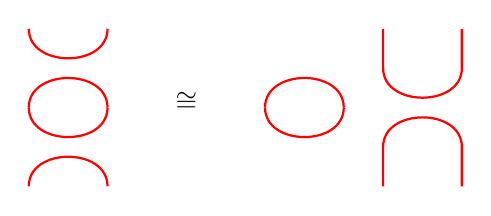
\begin{tikzpicture}
			\draw[thick, red] (0,2) .. controls (0,1.5) and (1,1.5) .. (1,2);
			\draw[thick, red] (0,1) .. controls (0,1.5) and (1,1.5) .. (1,1);
			\draw[thick, red] (0,0) .. controls (0,0.5) and (1,0.5) .. (1,0);
			\draw[thick, red] (0,1) .. controls (0,0.5) and (1,0.5) .. (1,1);
			\node[label={\(\cong\)}] at (2,0.7) {};
			\draw[thick, red] (3,1) .. controls (3,1.5) and (4,1.5) .. (4,1);
			\draw[thick, red] (3,1) .. controls (3,0.5) and (4,0.5) .. (4,1);
			\draw[thick, red] (4.5,0) to (4.5,0.5) .. controls (4.5,1) and (5.5,1) .. (5.5,0.5) -- (5.5,0);
			\draw[thick, red] (4.5,2) to (4.5,1.5) .. controls (4.5,1) and (5.5,1) .. (5.5,1.5) -- (5.5,2);
		\end{tikzpicture}}\par\bigskip
	\subcaptionbox{\(\U_3\U_1 = \U_1\U_3\)}{
		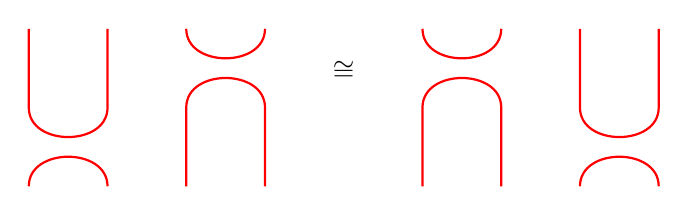
\begin{tikzpicture}
			\draw[thick, red] (0,0) .. controls (0,0.5) and (1,0.5) .. (1,0);
			\draw[thick, red] (0,2) -- (0,1) .. controls (0,0.5) and (1,0.5) .. (1,1) -- (1,2);
			\draw[thick, red] (2,0) -- (2,1) .. controls (2,1.5) and (3,1.5) .. (3,1) -- (3,0);
			\draw[thick, red] (2,2) .. controls (2,1.5) and (3,1.5) .. (3,2);
			\node[label={\(\cong\)}] at (4,1.1) {};
			\draw[rotate around={180:(5.5,1)}, xshift=5cm, thick, red] (0,0) .. controls (0,0.5) and (1,0.5) .. (1,0);
			\draw[rotate around={180:(5.5,1)}, xshift=5cm, thick, red] (0,2) -- (0,1) .. controls (0,0.5) and (1,0.5) .. (1,1) -- (1,2);
			\draw[rotate around={180:(7.5,1)}, xshift=5cm, thick, red] (2,0) -- (2,1) .. controls (2,1.5) and (3,1.5) .. (3,1) -- (3,0);
			\draw[rotate around={180:(7.5,1)}, xshift=5cm, thick, red] (2,2) .. controls (2,1.5) and (3,1.5) .. (3,2);
		\end{tikzpicture}}
	\caption{Input-output form relations}
	\label{fig:inputoutputillus}
\end{figure}

Now that we have the Temperley--Lieb algebra, we can define a mapping \[\uprho \colon \B_n \rightarrow \TL_n\] by the following formulae.
\begin{align*}
	\uprho (\sigmaa_i) &= A + A^{-1}\U_i,\\
	\uprho (\sigmaa_i^{-1}) &= A^{-1} + A\U_i.
\end{align*}
We see that \(\uprho\) is indeed a representation by verifying that \(\uprhoo(\sigmaa_i)\uprhoo(\sigmaa_i^{-1}) = 1\), \(\uprhoo(\sigmaa_i \sigmaa_{i+1} \sigmaa_i) = \uprhoo(\sigmaa_{i+1} \sigmaa_i \sigmaa_{i+1})\) and if  \(\abs{i-j} \geq 2\), \(\uprhoo(\sigmaa_i\sigmaa_j) = \uprhoo(\sigmaa_j\sigmaa_i)\).
\begin{prop}
	\(\uprhoo \colon \B_n \rightarrow \TL_n\) is a representation of the Artin braid group.
\end{prop}
\begin{proof}
	We first prove that \(\uprhoo(\sigmaa_i)\uprhoo(\sigmaa_i^{-1}) = 1\).
	\begin{align*}
		\uprhoo(\sigmaa_i)\uprhoo(\sigmaa_i^{-1}) &= (A + A^{-1}\U_i)(A^{-1} + A\U_i)\\
		&= 1 + (A^{-2} + A^2)\U_i + \U_i^2\\
	\end{align*}
	But since \(\U_i^2 = \updelta \U_i\) and \(\updelta = -A^{-2} - A^{2}\), we have
	\begin{align*}
		\uprhoo(\sigmaa_i)\uprhoo(\sigmaa_i^{-1}) &= 1 + (A^{-2} + A^2)\U_i + \updelta\U_i\\
		&= 1 + (A^{-2} + A^2) \U_i + (-A^{-2} - A^{2})\U_i\\
		&= 1.
	\end{align*}
	We now prove that \(\uprhoo(\sigmaa_i \sigmaa_{i+1} \sigmaa_i) = \uprhoo(\sigmaa_{i+1} \sigmaa_i \sigmaa_{i+1})\).
	\begin{align*}
		\uprhoo(\sigmaa_i \sigmaa_{i+1} \sigmaa_i) &= (A + A^{-1}\U_i)(A + A^{-1}\U_{i+1})(A + A^{-1}\U_i)\\
		&= (A^2 + \U_{i+1} + \U_i + A^{-2}\U_i\U_{i+1})(A + A^{-1}\U_i)\\
		&= A^3 + A\U_{i+1} + A\U_i + A^{-1}\U_i\U_{i+1} + A^{-2}\U_i^2 + A\U_i\\
		&\phantom{=} + A^{-1}\U_{i+1}\U_i + A^{-3}\U_i\U_{i+1}\U_i\\
		&= A^3 + A\U_{i+1} + (A^{-1}\updelta + 2A)\U_i\\
		&\phantom{=} + A^{-1}(\U_i\U_{i+1} + \U_{i+1}\U_i) + A^{-3}\U_i\\
		&= A^3 + A\U_{i+1} + (A^{-1}(-A^2 - A^{-2}) + 2A + A^{-3})\U_i\\
		&\phantom{=}+ A^{-1}(\U_i\U_{i+1} + \U_{i+1}\U_i)\\
		&= A^3 + A(\U_{i+1} + \U_i) + A^{-1}(\U_i\U_{i+1} + \U_{i+1}\U_i).
	\end{align*}
	Since symmetry of the above expression in \(i\) and \(i+1\), we can conclude that \(\uprhoo(\sigmaa_i \sigmaa_{i+1} \sigmaa_i) = \uprhoo(\sigmaa_{i+1} \sigmaa_i \sigmaa_{i+1})\).
	We now prove that if  \(\abs{i-j} \geq 2\), then \(\uprhoo(\sigmaa_i\sigmaa_j) = \uprhoo(\sigmaa_j\sigmaa_i)\).
	\begin{align*}
		\uprhoo(\sigmaa_i\sigmaa_j) &= \uprhoo(\sigmaa_i)(\sigmaa_j)\\
		&= (A + A^{-1}\U_i)(A + A^{-1}\U_j)
	\end{align*}
	Now since \(\U_i\U_j = \U_j\U_i\) if \(\abs{i-j} \geq 2\), we have \((A + A^{-1}\U_i)(A + A^{-1}\U_j) = (A + A^{-1}\U_j)(A + A^{-1}\U_i)\) which equals \(\uprhoo(\sigmaa_j\sigmaa_i)\).
\end{proof}

We now define the diagrammatic trace \(\tr \colon \TL_n \rightarrow \Z[A, A^{-1}]\) by extending linearly \(\tr(P) = \braket<P\,>\), where \(P\) is a product term in \(S(b)\). This version of trace is diagrammatic in nature as we are counting loops in a state. We thus arrive at the formula \(\braket<b> = \tr(\operatorname{\uprho}(b))\). With what we have learnt so far, one can now find a braid representation \(b\) of a link \(L\) by Alexander's theorem, calculate \(\tr(\operatorname{\uprho}(b))\) and normalise it to get the link invariant normalised bracket polynomial. One can substitute \(A = t^{-1/4}\) to arrive at our long sought destination of the Jones polynomial.

\section{Jones algebra}

Jones considered a sequence of algebras \(A_n\) for \(n = 2,3,\ldots\) with multiplicative generators \(e_1, e_2,\ldots, e_{n-1}\) and the following relations.
\begin{enumerate}
    \item \(e_i^2 = e_i\).
	\item \(e_ie_{i\pm 1} e_i = ce_i\).
	\item \(e_ie_j = e_je_i\) if \(\abs{i-j} \geq 2\).
\end{enumerate}
Here, \(c\) is a scalar which commutes with all the other elements. We can consider \(A_n\) as the free additive algebra on these generators viewed as a module over the ring \(\symbb{C}[c,c^{-1}]\), i.e.\@ we take the free ring in the generators \(e_1\), \(e_2\),\ldots, \(e_{n-1}\) and quotient it with the smallest ideal containing the elements \(e_i\), \(c^{-1}e_i e_{i+1}\) and \(e_i e_j e_i^{-1} e_j^{-1}\) with appropriately restricted \(i\) and \(j\). While \(c\) is often taken to be a complex number, we can view is as another algebraic variable which commutes with the generators. \(A_n\) arose in the theory of classification of von Neumann algebras and one can realize \(A_n\) as a von Neumann algebra as well. The reader is requested to compare the above mentioned relations for Jones algebra with the relations for the Artin braid group and the Temperley--Lieb algebra.

As mentioned in the beginning of this chapter, it is natural to construct a nested tower of algebras \[M_0 \hookrightarrow M_1 \hookrightarrow M_2 \hookrightarrow M_3\hookrightarrow \cdots \hookrightarrow M_n \hookrightarrow M_{n+1} \hookrightarrow\ldots\] with the following properties.
\begin{enumerate}
    \item \(M_0\) and \(M_1\) are given.
	\item \(e_i\colon M_i \rightarrow M_{i-1}\) is a `projection'.
	\item \(e_i^2 = e_i\).
	\item \(M_{i+1} = \left\langle M_i,e_i\right\rangle\).
\end{enumerate}
Jones constructed such a tower of algebras with the other two properties of generators \(e_ie_{i\pm 1} e_i = ce_i\) and \(e_ie_j = e_je_i\) if \(\abs{i-j} \geq 2\). He defined a notion of a trace \(\tr\colon M_n \rightarrow \C\), i.e.\@ a function which vanishes on the commutator of any two elements of \(M_n\). This trace satisfied so called Markov property: \(\tr(we_i) = c\tr(w)\) for \(w\) in the algebra generated by \(M_0\), \(e_i\),\ldots, \(e_{i-1}\).

We now see a concrete example of such a tower of algebras. Consider \[\R \hookrightarrow \R[x_1] \hookrightarrow \R[x_1, x_2] \hookrightarrow \R[x_1, x_2, x_3] \hookrightarrow \cdots \hookrightarrow \R[x_1, x_2, \ldots, x_n] \hookrightarrow \ldots.\] We have a sequence of the set of all real numbers, the set of all real polynomials in one variable, the set of all real polynomials in two variables, the set of all real polynomials in three variables, and so on. Each variable \(x_i\) for \(i\geq 2\), is a map from \(\R[x_1, x_2, \ldots, x_{i-1}]\) to \(\R[x_1, x_2, \ldots, x_{i-2}]\), defined as the coefficient of \(x_{i-1}^0 \in \R[x_1, x_2, \ldots, x_{i-1}]\).
\begin{align*}
	x_i &\colon \R[x_1, x_2, \ldots, x_{i-1}] \rightarrow \R[x_1, x_2, \ldots, x_{i-2}]\\
	x_i &\colon \sum_{j=0}^{m}p_j x^{j}_{i-1} \mapsto p_0,
\end{align*}
where \(p_j \in \R[x_1, x_2, \ldots, x_{i-2}]\) and \(m\in\n\). As an example, if \(\sum_{j=0}^{m}p_j x^{j}_1 \in \R[x_1]\), then
\begin{align*}
    x_2 &\colon \R[x_1] \rightarrow \R\\
	x_2 &\colon \sum_{j=0}^{m}p_j x^{j}_1 \mapsto p_0,
\end{align*}
where \(p_0\) is the coefficient of \(x_1^0\), i.e.\@ the constant term. For example, \[x_2 (3x_1^4 + 6x_1^3 + x_1 + 5) = 5.\] Similarly, \(x_3\) is a map from \(\R[x_1, x_2]\) to which maps a polynomial in two variables to the polynomial (in the single variable \(x_1\)) which does not contain any power of \(x_2\). As an example, \[x_3(4x_1x_2^2 + 3x_1^3 + x_2 + x_2^5 + 1) = 3x_1^3 + 1.\]

\((\R[x_1, x_2, \ldots, x_n], +, \cdot)\) is an algebra with \(+\) defined as polynomial addition (component-wise addition) and \(\cdot\) defined as  polynomial multiplication (Cauchy product). The generator relations for the Jones algebra, however, are not satisfied with the \(\cdot\) operation; \(x_1^2 \coloneq x_1 \cdot x_1 \neq x_1\). But we can make sense of them if we interpret the operation amongst the generators as the function composition operator. \(x_1\), \(x_2\),\ldots, \(x_n\) are the generators \((\R[x_1, x_2, \ldots, x_n], +, \cdot)\). Since \(x_i\)'s are functions as well, we can interpret \(x_i^2\) as \(x_i \circ x_i\). If we do that, then \(x_i^2 \coloneq x_i \circ x_i = x_i\) as \(x_i\) is a projection operator. Similarly, we see that \(x_i \circ x_{i\pm 1}\circ x_i = x_i\) and \(x_i \circ x_j = x_j \circ x_i\) by restricting the domains appropriately.

We can define a Markov trace on the above tower as follows. For an element \(w \in \R[x_1, x_2, \ldots, x_{n}]\), define \(\tr \colon \R[x_1, x_2, \ldots, x_{n}] \rightarrow \Z\) by assigning \(w\) the degree of the polynomial. For an element of \(\R[x_1, x_2, \ldots, x_{n+1}]\), \(\tr \colon \R[x_1, x_2, \ldots, x_{n+1}] \rightarrow \Z\). Even though the domains of the trace are different in the above two examples, we can perform this abuse of notation since there is no risk of confusion here. We see that \(\tr(w x_{n+1}) = \tr(w)\). Thus, \(\tr\) is a Markov trace as it satisfies the Markov property with \(c=1\) for all \(w \in \R[x_1, x_2, \ldots, x_{n}]\) where \(n \geq 1\).

We can retrieve the Jones algebra from the Temperley--Lieb algebra by substituting \(e_i = \updelta^{-1} \U_i\), \(e_i^2 = e_i\) and \(e_ie_{i\pm 1} e_i = \updelta^{-2}e_i\). We have taken \(c = \updelta^{-2}\). Note that the underlying rings are different.

